\documentclass[letterpaper, inpress]{jds} % use this for production

% \documentclass[a4paper, review]{jds}      % use this for review


%%%%%%%%%%%%%%%%%%%%%%%%%%%%%%%%%%%%%%%%%%%%%%%%%%%%%%%%%%%%%%%%%%%%%%
%% the following edits should be done by Journal typesetters
%%%%%%%%%%%%%%%%%%%%%%%%%%%%%%%%%%%%%%%%%%%%%%%%%%%%%%%%%%%%%%%%%%%%%%
\setcounter{page}{1}            % set the first page number
\jdsmonth{July}                 % month
\jdsyear{2023}                  % year
\jdsvolume{xx}                  % volume number
\jdsissue{xx}                   % issue number
\jdsdoi{xx.xxxx/xxxxxxxxx}      % doi
\jdsreceived{July, 2023}       % optional: comment it out if no received date
\jdsaccepted{August, 2023}         % optional: comment it out if no accepted date
%% manually set running header for a shorter list of authors if needed
% \shortauthors{A Author A, et al.}


%%%%%%%%%%%%%%%%%%%%%%%%%%%%%%%%%%%%%%%%%%%%%%%%%%%%%%%%%%%%%%%%%%%%%%
%% edits by authors are given below
%%%%%%%%%%%%%%%%%%%%%%%%%%%%%%%%%%%%%%%%%%%%%%%%%%%%%%%%%%%%%%%%%%%%%%
\usepackage{listings}
\lstset{language=R,frame=tlb,float} 
\usepackage[x11names, svgnames, rgb]{xcolor}
\usepackage[utf8]{inputenc}
\usepackage{tikz}
\usetikzlibrary{snakes,arrows,shapes}
\usepackage{amsfonts,amsmath,amssymb,amsthm}
\usepackage{booktabs}

\title{A Platform for Large Scale Statistical Modelling in \proglang{R}}

\author[1]{Jason Cairns\thanks{corresponding email:\href{mailto:jason.cairns@auckland.ac.nz}{jason.cairns@auckland.ac.nz}}}
\author[1]{Simon Urbanek}
\author[1]{Paul Murrell}
\affil[1]{Department of Statistics, University of Auckland, New Zealand}

\begin{document}

\maketitle

\begin{abstract}
With the growing scale of big datasets, fitting novel statistical models on larger-than-memory datasets becomes correspondingly challenging.
This document outlines the development and use of \pkg{largescaler}, a platform developed specifically for the development of statistical models for big datasets.
\end{abstract}
\begin{keywords} % alphabetical; excluding anything in the title already
Big Data;
Distributed Computing;
Modelling;
\end{keywords}

\section{Introduction}%
\label{sec:intro}

The rate of growth of datasets continues to outpace attempts to engage meaningfully with them, as individual computer memory limits are increasingly exceeded~\citep{kleppmann2017dataintensive}.
At the scale of big data, speed also becomes a constraining factor, with concurrency and parallelism being of increasing importance.
The aim of a statistician seeking to gain novel insight from such datasets commonly includes the interactive use of a complex statistical model, often implemented from scratch using \proglang{R}.
No single system satisfactorily provides the capacity to meet this demand.

Those systems that do come close to meeting the demand provide direction regarding how to gain insight from larger-than-memory datasets.
Most importantly, the standard solution for handling big data is to operate over a distributed system~\citep{boja2012distributed}.
Several systems have seen widespread use within the context of data and machine learning pipelines, such as \pkg{Spark}~\citep{zaharia2016apache} and \pkg{Hadoop Map-Reduce}~\citep{shvachko2010hadoop}.
For the statistician mostly familiar with \proglang{R}, these systems provide API's to \proglang{R} where distributed data may be manipulated and pre-made models fitted.
However, these API's are often found lacking when attempted to be used for the creation of complex statistical models that don't come pre-packaged, due to this not being their primary use-case, and \proglang{R} not being their target language.

For instance, \pkg{sparklyr} is an interface to Spark from within R~\citep{luraschi20}.
The user connects to spark and accumulates instructions for the manipulation of a \pkg{Spark} DataFrame object using \pkg{dplyr} commands, then executing the request on the \pkg{Spark} cluster.
It works fluidly when intentions meet the \pkg{Spark} paradigm, but due to it being only an interface to an external system, it is commonly required to program directly to \pkg{Spark} specifications, using \proglang{Scala}, when more complex and custom analyses are required.

The most notable general interface in \proglang{R} that has capabilities for large data is the the \pkg{foreach} package~\citep{microsoft20}.
The backends are provided by other packages, typically named with some form of ``Do\emph{X}'', and can be drivers to external or \proglang{R}-specific systems.
Parallelisation is enabled by some backends, with \pkg{doParallel} allowing parallel computations~\citep{corporation19}, \pkg{doSNOW} enabling cluster access through the \pkg{SNOW} package~\citep{dosnow19}, and \pkg{doMPI} allowing for direct MPI access~\citep{weston17}.
\pkg{foreach} remains an exceptional and general interface, but can only be as performant as the backend driver packages.
The necessity of persisting large data objects and allowing for complex manipulation of them is not met by any of the reviewed package backends.

The most complete self-contained interface that was developed specifically for statistical modelling in \proglang{R} is given by the \pkg{pbdR} collection.
This collection allows for for distributed computing with \proglang{R}~\citep{pbdBASEpackage}, with the name being the abbreviation of Programming with Big Data in R.
The packages include high-performance communication and computation capabilities, including \pkg{RPC}, \pkg{ZeroMQ}, and \pkg{MPI} interfaces.
The collection is extensive, offering several packages for each of the main categories of application functionality, communication, computation, development, I/O, and profiling.
While incredibly performant and great care has been taken to provide an interface as close to native \proglang{R} as possible, the provided packages still require an MPI form of shared program amongst all cluster nodes, which presents an unfamiliar form of program specification to most \proglang{R} users.
In addition, more complex analyses requiring lower-level data manipulation end up increasingly involved with the complexities of MPI, which was authored as a far more general system than its use-case in \pkg{pbdR}, thereby possessing a far greater complexity than necessitated.
Regardless, the direction provided of distributing large data across compute nodes, as a means of statistical interaction, is a concept that has been proven well by this package collection.

Within the motivating context provided, the \pkg{largescaler} project has sought to provide a full stack for working with larger-than-memory data in \proglang{R}, allowing the developer to manipulate distributed data and create arbitrarily complex iterative models with which to fit to the data, over a self-contained user-specified computing cluster. Further details on \pkg{largescaler} are provided in~\citet{cairns2023}.

\section{Construction of a Large-Data Statistical System API for R}

The construction of such \pkg{largescaler} has roots in a theoretical reconsideration of precisely what determines the necessary components of a system capable of complex statistical modelling with larger-than-memory data in a distributed fashion.
The structure of such considerations have been defined principally by the response to linguistic challenges facing such an API.

In order to perform calculations on larger-than-memory data, we need some means of \textbf{representing} the data, in order for it to be tangible and useful.
All objects, regular or irregular, are facilitated in their access and manipulation by way of an \textbf{object system}, which is an organised manner of interaction with objects.
We choose the description of an object system as the basis for the theoretical development of our project as it is that aspect which is most proximal to the constraint imposed by the scale of data dealt with, in being that aspect which defines how data is dealt with.
The central constraint is that the data is larger than computer memory.
This, coupled with the fact that they must be worked on in-memory, leads to an impossible design if combined naively.
The only possible means is to split the data into smaller pieces that do fit in memory.
Such a structure, common among big data systems, is known as a shard, or a \textbf{chunk}. 
The chunk thus serves as the lowest level object manipulable by the user, and defines the lower level of the layered object system.
The end-user is typically not interested in the chunks making the object.
Therefore higher-level objects are introduced as compositions of chunks, serving as abstract collections where individual chunks are a layer of concern below the user interface.
Such higher-level objects are termed \textbf{distributed objects}, and serve as the primary data structure interacted with by the high-level user, with a representative example depicted in Figure~\ref{fig:distobj}.

\begin{figure}[ht]
\begin{center}
    
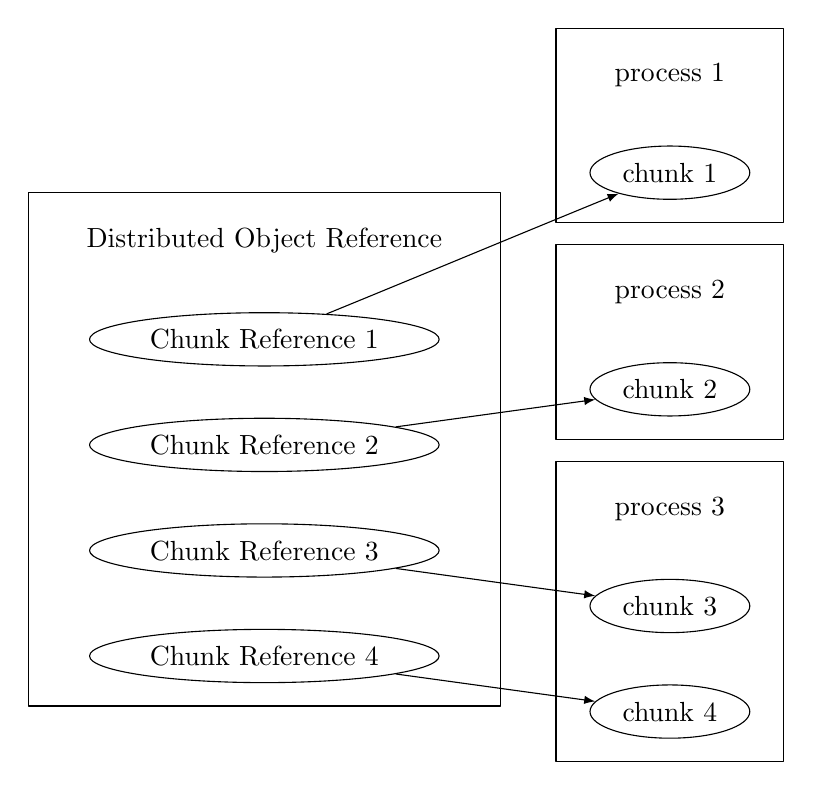
\begin{tikzpicture}[>=latex,line join=bevel,]
%%
\begin{scope}
  \pgfsetstrokecolor{black}
  \definecolor{strokecol}{rgb}{0.0,0.0,0.0};
  \pgfsetstrokecolor{strokecol}
  \draw (0.0bp,28.0bp) -- (0.0bp,213.0bp) -- (170.0bp,213.0bp) -- (170.0bp,28.0bp) -- cycle;
  \draw (85.0bp,195.5bp) node {Distributed Object Reference};
\end{scope}
\begin{scope}
  \pgfsetstrokecolor{black}
  \definecolor{strokecol}{rgb}{0.0,0.0,0.0};
  \pgfsetstrokecolor{strokecol}
  \draw (190.0bp,202.0bp) -- (190.0bp,272.0bp) -- (272.0bp,272.0bp) -- (272.0bp,202.0bp) -- cycle;
  \draw (231.0bp,255.0bp) node {process 1};
\end{scope}
\begin{scope}
  \pgfsetstrokecolor{black}
  \definecolor{strokecol}{rgb}{0.0,0.0,0.0};
  \pgfsetstrokecolor{strokecol}
  \draw (190.0bp,124.0bp) -- (190.0bp,194.0bp) -- (272.0bp,194.0bp) -- (272.0bp,124.0bp) -- cycle;
  \draw (231.0bp,177.0bp) node {process 2};
\end{scope}
\begin{scope}
  \pgfsetstrokecolor{black}
  \definecolor{strokecol}{rgb}{0.0,0.0,0.0};
  \pgfsetstrokecolor{strokecol}
  \draw (190.0bp,8.0bp) -- (190.0bp,116.0bp) -- (272.0bp,116.0bp) -- (272.0bp,8.0bp) -- cycle;
  \draw (231.0bp,99.0bp) node {process 3};
\end{scope}
  \node (cr1) at (85.0bp,160.0bp) [draw,fill=white,ellipse] {Chunk Reference 1};
  \node (cr2) at (85.0bp,122.0bp) [draw,fill=white,ellipse] {Chunk Reference 2};
  \node (cr3) at (85.0bp,84.0bp) [draw,fill=white,ellipse] {Chunk Reference 3};
  \node (cr4) at (85.0bp,46.0bp) [draw,fill=white,ellipse] {Chunk Reference 4};
  \node (c1) at (231.0bp,220.0bp) [draw,fill=white,ellipse] {chunk 1};
  \node (c2) at (231.0bp,142.0bp) [draw,fill=white,ellipse] {chunk 2};
  \node (c3) at (231.0bp,64.0bp) [draw,fill=white,ellipse] {chunk 3};
  \node (c4) at (231.0bp,26.0bp) [draw,fill=white,ellipse] {chunk 4};
  \draw [->] (cr1) ..controls (133.86bp,179.94bp) and (175.11bp,197.13bp)  .. (c1);
  \draw [->] (cr2) ..controls (152.85bp,131.29bp) and (175.38bp,134.41bp)  .. (c2);
  \draw [->] (cr3) ..controls (152.85bp,74.715bp) and (175.38bp,71.586bp)  .. (c3);
  \draw [->] (cr4) ..controls (152.85bp,36.715bp) and (175.38bp,33.586bp)  .. (c4);
%
\end{tikzpicture}


\caption{Distributed object, showing chunks and their references across disparate nodes.}
\label{fig:distobj}
\end{center}
\end{figure}

With the establishment of an object system, attention may then be turned to the actualities of \textbf{computation}. 
For each chunk, each operation must possess the following properties:

\begin{itemize}
    \item Operations on chunks must have some means of access to all of the relevant chunk arguments to operate on together;
    \item The operation must have a stored description of some kind;
    \item The result of the operation must be stored somewhere.
\end{itemize}

A \textbf{chunk function applicator} is required that takes a function and some chunks, sending the operation to a node which apply the function to the specified chunks.
The applicator requires some means of access to the respective chunks.
An equivalent \textbf{distributed object function applicator} is to be defined in a similar manner, though for distributed objects.
Likewise, following the conclusion of the operation, some means of access to the result is required - the result is to be kept as a distributed object itself, allowing for further iterative action on it.

Some of the concerns relevent to the applicators include questions of argument sourcing and interaction.
With regards to sourcing, the optimal node should be chosen to perform the operation in order to minimise data movement.
All chunks not immediately available to the operating node are needed to be made so in order for the operation to take place.
Interaction between chunks, especially in the context of the distributed object function applicator, seeks to answer the question of how these distributed arguments are to be treated in multiple.
For instance, whether to recycle chunks, and how they are to be appropriately combined.

After laying out the distributed objects and the operations that they may be engaged in, we reach the limits of the construction of the system.
The mechanical aspects of the system developed, focus is turned to the more complex and precise notions of the arrangement of these components;
let us expand the construction limits now by exploring and describing the component of time as it relates to the system - specifically, \textbf{concurrency} within the system.
Here, we treat concurrency in the manner of \citet{pike2012concurrency}, where it is used to refer to the composition of independently executing processes.
Considering the system as a whole, and determining the independently executing processes within it and how they may be composed, it is clear that a distributed system has significant room for concurrency, which serves to aid speed and memory usage.
Assuming distinct nodes for performing operations on chunks, a remarkable thing would occur on the requesting client: nothing happens.
The processing occurs in an entirely separate memory space, with a different processor.
Were the client performing operations on regular, non-chunk objects, the processing would bind up the client, and it would block until the operation completed.
This recognition opens up a broad mix of possibilities and complications.
In terms of possibilities, the potential for chunk operations to be non-blocking to the client means that operations may be \textbf{asynchronous}, which would allow for significantly more efficient ordering of events within the system.
Long operations on chunks may take place side-by-side with client-side operations on local objects, neither interfering with each other. The converse of such a possibility is the new potential for \textbf{race conditions}, where the unordered timing of events may lead to undesirable behaviour. 

Through the defining feature of distributed data being incapable of direct reference, we have established that there must be some entity through which to indirectly interact with the distributed data.
This entity we have given the appellation of \textbf{`Distributed Object Reference'}, and serves as a proxy which is directly affected by the user in order to pass on further information to and from the distributed data which the reference refers to.
This relationship between the reference and the distributed data is known as \textbf{``adequacy''} in formal semantics, with the role of the distributed data as the object of indirect interaction being called the \textbf{``referent''} \citep{gordon1984}.
It must be established that the reference itself may be of conceptual interest.
The referents themselves, if completely transparent to a reference, possess no information on their relation to each other.
This information needs to be captured somewhere accessible to the user, with most distributed algorithms being dependent on the knowledge of how the underlying chunks relate, in dimension or quantity. 
Generalising the terminology of \citet{quine1979}, the distinction between the \textbf{use} and \textbf{mention} with respect to  distributed objects lies in the contrasting operations that may be intended of a distributed object reference: interaction may be intended for either the referent distributed object (use), or the reference itself (mention).
Such semantics of access to the reference and referent serve as the basis for much of metaprogramming, and may be considered a valuable component of a distributed statistical system.

\section{User Interface}\label{sec:ui}

\pkg{largescaler} serves as a functioning system, capable of performing complex statistical analyses over datasets spanning hundreds of nodes.
The implementation of this system makes use of a layered approach, wherein each layer targets a different category of user.
The \pkg{largescaler} interface is the principal new contribution by this project, delivering a novel means of interacting with distributed data through meaningful primitives defined at every level of abstraction.
A key offering of the layered approach is the ease by which a user of the package can traverse the levels as needed, with irrelevent information remaining hidden until required.
The levels of abstraction correspond to users of the package, given as the following:

\begin{description}
    \item[Analyst] A user solely interested in using the provided models and statistical functions in order to attain insight into some larger-than-memory data, typically a distributed data frame. All details of distribution are abstracted away.
    \item[Researcher] A user seeking to develop their own distributed statistical models. Distributed objects are to be considered as singular cohesive objects.
    \item[Developer] A user seeking greater expressivity in the definition of statistical models. Chunks are considered a relevant concern to be manipulated directly.
    \item[Architect] A user intending to directly modify the network topology of the distributed system, mainly in order to attain major efficiency gains.
\end{description}

Each of the users are served by the aforementioned packages making up the framework, in turn serving a logical layer of abstraction.
This mapping is given in Table \ref{tab:layer}.

\begin{table}[h!]
\centering
\caption{A mapping of logical layers, users and the respective packages provided by the \pkg{largescaler} framework to enable the use.}
\label{tab:layer}
\begin{tabular}{@{}lll@{}}
\toprule
Layer & User & Package \\ \midrule
Model Usage & Analyst & \pkg{largescalemodelr} \\
Model Description & Researcher & \pkg{largescaler} \\
Cluster Interaction & Developer & \pkg{chunknet} \\
Communication & Architect & \pkg{orcv} \\ \bottomrule
\end{tabular}
\end{table}

Owing to considerations of space, this description of the user interface will focus solely on the key offerings of the \pkg{largescaler} user interface, with descriptions of other components and packages having a fuller treatment in \citet{cairns2023}.
Use of the API is given by way of example below.

Consider first a simple operation of summation.
Consider some vector $x$ that is broken up into $j$ chunks, yielding $j$ subvectors of length $i$.
Due to associativity the sum of the whole is the sum of the sum of the parts, as shown in Equation \ref{eqn:sum}.

\begin{equation}\label{eqn:sum}
    \sum_i x_i= \sum_{j,i}x_{ij} = \sum_j\sum_i x_{ij}
\end{equation}

In an effort to maintain as close proximity as possible between the mathematical description and the provided interface, this may be written in \pkg{largescaler} in the form given by Listing \ref{lst:sum}

\begin{lstlisting}[caption={Distributed summation with largescaler},label={lst:sum}]
d(sum)(x) |>
emerge() |>
sum()
\end{lstlisting}

Here, the \lstinline{d()} applicator function transforms the base \lstinline{sum()} function to work over distributed objects, in this example given by \lstinline{x}.
\lstinline{sum()} is therefore sent to each chunk, yielding a new distributed object as the output.
This output distributed object can be brought back to the requesting client and combined using the provided \lstinline{emerge()} function, yielding a regular \proglang{R} numeric vector of sums.
This vector of sums may then be summed as normal, providing the final result.
The given example is actually a very simple application of map-reduce, and could effectively serve as the \lstinline{sum()} method for distributed objects

Consider something slightly more complex: the arithmetic mean.
Again, using a chunked mathematical description as given in Equation \ref{eqn:mean}, a related means of specification through \pkg{largescaler} is possible, given in Listing \ref{lst:mean}.

\begin{equation}\label{eqn:mean}
    \overline{x} = \frac{\sum_{i}x_{i}}{n} = \frac{\sum_{j,i}x_{ij}}{\sum_j n_j}
\end{equation}

\begin{lstlisting}[caption={Distributed arithmetic mean with largescaler},label={lst:mean}]
sum(x) / { 
	d(length)(x) |> 
	sum()
}
\end{lstlisting}

Here we build on the distributed sum introduced above, but the total length of The distributed object is relevent as the denominator.
Assuming a \lstinline{sum()} method for distributed objects as described, and math methods defined in a similar fashion, the denominator is defined using the same \lstinline{d()} function that sends a \lstinline{length} computation to all of the chunks.

Finally, consider the cumulative sum.
It is important in this case to think of chunks as being in series, which is determined by the structure of the distributed object reference.
The main difference between a non-distributed and a distributed version of cumulative sum is that for each chunk in the series, computation requires the cumulative sum of the previous chunk as a starting value.
Using a chunked mathematical description, cumulative sum may be described by Equation \ref{eqn:cumsum}.

\begin{equation}
\begin{gathered}\label{eqn:cumsum}
    S_i = S_{i-1}+x_i, \quad S_0 = 0\\
    \iff S_{i,j} = S_{i-1,j} + x_{i,j}, \quad S_{0,j} = S_{n_i,j-1},\\
    \qquad S_{0,0} = 0
\end{gathered}
\end{equation}

This can be expressed in a functional manner using the \textit{reduce} operator, also known as a \textit{fold}, and the \pkg{largescaler} framework provides a distributed form of such a function, where the results of one chunk are sent as the initial value to the reduce function as applied to the next chunk and so on in series.
An example of a reduce operation is given in Figure \ref{fig:dreduce}.

\begin{figure}[ht]
\begin{center}
    
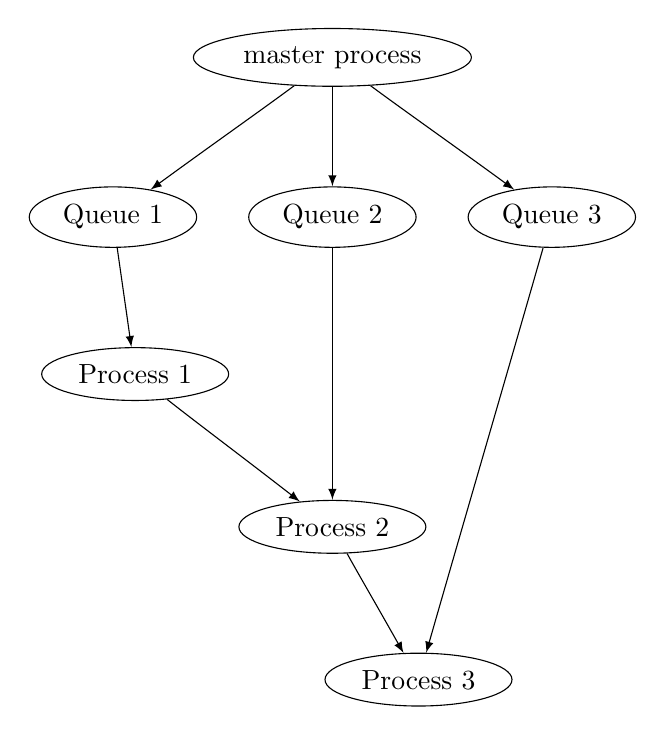
\begin{tikzpicture}[>=latex,line join=bevel,]
%%
\begin{scope}
  \pgfsetstrokecolor{black}
  \definecolor{strokecol}{rgb}{1.0,1.0,1.0};
  \pgfsetstrokecolor{strokecol}
  \definecolor{fillcol}{rgb}{1.0,1.0,1.0};
  \pgfsetfillcolor{fillcol}
  \filldraw (0.0bp,0.0bp) -- (0.0bp,244.0bp) -- (219.0bp,244.0bp) -- (219.0bp,0.0bp) -- cycle;
\end{scope}
\begin{scope}
  \pgfsetstrokecolor{black}
  \definecolor{strokecol}{rgb}{1.0,1.0,1.0};
  \pgfsetstrokecolor{strokecol}
  \definecolor{fillcol}{rgb}{1.0,1.0,1.0};
  \pgfsetfillcolor{fillcol}
  \filldraw (0.0bp,0.0bp) -- (0.0bp,244.0bp) -- (219.0bp,244.0bp) -- (219.0bp,0.0bp) -- cycle;
\end{scope}
  \node (q1) at (30.5bp,176.0bp) [draw,ellipse] {Queue 1};
  \node (q2) at (109.5bp,176.0bp) [draw,ellipse] {Queue 2};
  \node (q3) at (188.5bp,176.0bp) [draw,ellipse] {Queue 3};
  \node (m) at (109.5bp,233.5bp) [draw,ellipse] {master process};
  \node (p1) at (38.5bp,119.5bp) [draw,ellipse] {Process 1};
  \node (p2) at (109.5bp,64.5bp) [draw,ellipse] {Process 2};
  \node (p3) at (140.5bp,9.5bp) [draw,ellipse] {Process 3};
  \draw [->] (m) ..controls (84.261bp,214.77bp) and (65.841bp,201.83bp)  .. (q1);
  \draw [->] (m) ..controls (109.5bp,215.84bp) and (109.5bp,206.15bp)  .. (q2);
  \draw [->] (m) ..controls (134.74bp,214.77bp) and (153.16bp,201.83bp)  .. (q3);
  \draw [->] (q1) ..controls (33.033bp,157.74bp) and (34.506bp,147.71bp)  .. (p1);
  \draw [->] (q2) ..controls (109.5bp,146.51bp) and (109.5bp,107.36bp)  .. (p2);
  \draw [->] (q3) ..controls (177.57bp,137.55bp) and (156.0bp,63.62bp)  .. (p3);
  \draw [->] (p1) ..controls (60.126bp,102.36bp) and (77.076bp,89.704bp)  .. (p2);
  \draw [->] (p2) ..controls (118.86bp,47.493bp) and (125.03bp,36.954bp)  .. (p3);
%
\end{tikzpicture}


\caption{Example distributed reduce pattern from controlling process.}
\label{fig:dreduce}
\end{center}
\end{figure}

This is put to use for cumulative sum by \pkg{largescaler} as in Listing \ref{lst:cumsum}.

\begin{lstlisting}[caption={Distributed cumulative sum with largescaler},label={lst:cumsum}]
dReduce(cumsum, x) |>
emerge() 
\end{lstlisting}

A distributed object is returned that by default just holds the final accumulation, consisting of one single chunk.

\section{Discussion/Conclusions}

The \pkg{largescaler} system has been proven over a number of application areas.
Data manipulation is a basic necessity, as it is required for modelling, and is provided well by other systems.
\pkg{largescaler} is capable of a full set of data manipulations, including all that are provided by the \pkg{dplyr} package.
Model fitting is demonstrated in the proof-of-concept \pkg{largescalemodelr} package, which includes a variety of models, including linear models and generalised linear models.
Work is currently underway to develop examples of boosted models, as well as a convex optimisation methods such as the alternating direction method of multipliers.

Initial benchmarking results are highly promising, with performance results measuring not only speed but capability;
One instance of capability is given in the creation of a contingency table of a large dataset that crashed \proglang{Spark} but was computed in several seconds using \pkg{largescaler}.

The scope for future work remains significant, enabled by the high level of extensibility provided by the system.
External systems which serve to monitor performance or take up the role of garbage collection would grant the possibility of greater reliabilit.
Robustness could be gained through self-healing datasets, a potential that has a precedent in a current prototype, which allows for resiliance to node failure in a more efficient manner than that of the current Resilient Distributed Datasets~\citep{zaharia2012resilient}.
Further resiliance can be gained within the system through operating the location service as a distributed hash table, leaving no central point of failure in a fully peer-to-peer system.

\bibliographystyle{jds}
\bibliography{largescaler-jason-cairns}

\end{document}